\documentclass[12pt, twoside]{article}
% \documentclass[12pt, twoside]{article}
\usepackage[letterpaper, margin=1in, headsep=0.2in]{geometry}
\setlength{\headheight}{0.6in}
%\usepackage[english]{babel}
\usepackage[utf8]{inputenc}
\usepackage{microtype}
\usepackage{amsmath}
\usepackage{amssymb}
%\usepackage{amsfonts}
\usepackage[nomessages]{fp} %\FPeval{\var-name}{2*sin(pi/6)}
\usepackage{siunitx} %units in math. eg 20\milli\meter
\usepackage{yhmath} % for arcs, overparenth command
\usepackage{tikz} %graphics
\usetikzlibrary{quotes, angles, arrows, arrows.meta}
\usepackage{graphicx} %consider setting \graphicspath{{images/}}
\usepackage{parskip} %no paragraph indent
\usepackage{enumitem}
\usepackage{multicol}
\usepackage{venndiagram}

\usepackage{fancyhdr}
\pagestyle{fancy}
\fancyhf{}
\renewcommand{\headrulewidth}{0pt} % disable the underline of the header
\raggedbottom
\hfuzz=2mm %suppresses overfull box warnings

\usepackage{hyperref}
\usepackage{float}

\title{Algebra 2}
\author{Chris Huson}
\date{September 2024}

\fancyhead[LE]{\thepage}
\fancyhead[RO]{\thepage \\ First and last name: \hspace{2.5cm} \,\\ Section: \hspace{2.5cm} \,}
\fancyhead[LO]{BECA/Huson/Precalculus: Sequences \\* 19 September 2024}

\begin{document}
\subsubsection*{1.12 Test: Powers and radicals, sequences \hfill Mental math - no calculators}
\begin{enumerate}[itemsep=0.5cm]

\item Memorize the squares to 100. \hfill \emph{3.OA.7 Fluently multiply and divide within 100}
    \begin{multicols}{2}
        \begin{enumerate}[itemsep=0.5cm]
            \item $3^2 =$
            \item $9^2 =$
            \item $6^2 =$
            \item $3^3 =$
        \end{enumerate}
    \end{multicols}

\item Memorize the square roots of whole numbers through 100 and cubes through five.
    \begin{multicols}{2}
        \begin{enumerate}[itemsep=0.5cm]
            \item $\sqrt{64} =$
            \item $\sqrt{16} =$
            \item $\sqrt{49} =$
            \item $\sqrt{4} =$
            \item $\sqrt[3]{27} =$
            \item $\sqrt[3]{8} =$
          \end{enumerate}
    \end{multicols}

\item Round to the \emph{nearest thousandth}.
  \begin{multicols}{2}
  \begin{enumerate}[itemsep=1.5cm]
    \item $A=3.1415926$
    \item $V=1.4142135$
  \end{enumerate}
  \end{multicols} \vspace{0.5cm}

\item Simplify each expression by ``collecting like terms''
\begin{enumerate}[itemsep=2cm]
  \begin{multicols}{2}
    \item $x-5x^2-6x+9x^2$
    \item $5\sqrt{3}+3y-\sqrt{3}-7y$
  \end{multicols}
  \end{enumerate} \vspace{1cm}

\item Use the function $f(x) = 3x-5$ to answer the questions.
  \begin{multicols}{2}
  \begin{enumerate}[itemsep=2cm]
      \item What is $f(1)$?
      \item Find $f(\frac{2}{3})$
      \item Solve for $x$ if $f(x) = 16$.
  \end{enumerate}
  \end{multicols} \vspace{1cm}

\newpage

% June 2019 Regents - Problem 8
\item Which sequence is defined recursively?
\begin{enumerate}
    \item $a_n = 4n - 5$
    \item $a_n = n^2 + 2$
    \item $a_1 = 16$ and $a_n = a_{n-1} \times \frac{1}{2}$
    \item $a_n = 1 + \frac{1}{2}n$
\end{enumerate}


% August 2019 Regents - Problem 12
\item The nth term of a sequence is given by $a_n = 5n - 3$. What is the 10th term of the sequence?
\begin{enumerate}
    \item 47
    \item 45
    \item 43
    \item 41
\end{enumerate}

% January 2019 Regents - Problem 16
\item A sequence is defined recursively by $ a_1 = 5 $ and $ a_{n+1} = 2a_n$ for $ n \geq 1 $. Find the first four terms of the sequence. \vspace{2cm}

% Example Problem 3
\item A geometric sequence has a first term of $a_1 = 4$ and a common ratio of $r = \frac{1}{2}$. Write the recursive formula for the sequence. Calculate the 5th term. \vspace{4cm}

\item Write a recursive formula for the sequence $1, 3, 9, 27, \dots$ \vspace{2cm}


\newpage

% June 2019 Regents - Problem 10
\item Which situation could be modeled using a geometric sequence?
\begin{enumerate}
    \item A cell phone company charges \$30.00 per month for 2 gigabytes of data and \$12.50 for each additional gigabyte of data.
    \item The temperature in your car is $79^\circ$. You lower the temperature of your air conditioning by $2^\circ$ every 3 minutes in order to find a comfortable temperature.
    \item David's parents have set a limit of 50 minutes per week that he may play online games during the school year. However, they will increase his time by 5\% per week for the next ten weeks.
    \item Sarah has \$100.00 in her piggy bank and saves an additional \$15.00 each week.
\end{enumerate}

\item Which of the following is the recursive formula for the sequence $40, 30, 20, \ldots$
  \begin{multicols}{2}
  \begin{enumerate}
    \item $g_n = 40 -10(n-1)$
    \item $g_1 = 40$ \\ $g_n = g_{n-1} -10$
    \item $g_n = 40 \left( \frac{3}{4} \right)^{n-1}$
    \item $g_1 = 40$ \\ $g_n = \frac{3}{4} g_{n-1}$
  \end{enumerate}
  \end{multicols}

% January 2019 Regents - Problem 24
\item A sequence is defined recursively by $a_1 = 3$ and $a_{n+1} = 2a_n - 1$ for $n \geq 1$. What is the explicit formula for the nth term of the sequence? %Challenge
\begin{enumerate}
    \item $a_n = 2^n - 1$
    \item $a_n = 2^n + 1$
    \item $a_n = 3 \cdot 2^{n-1}$
    \item $a_n = 3 \cdot 2^n - 1$
\end{enumerate}

\item A tree farm initially has 150 trees. Each year, 20\% of the trees are cut down and 80 seedlings are planted. Which recursive formula models the number of trees, $a_n$, after $n$ years? %January 2023 Regents
\begin{enumerate}
    \item $a_1 = 150$ \\ $a_n = a_{n-1}(0.2) + 80$
    \item $a_1 = 150$ \\ $a_n = a_{n-1}(0.8) + 80$
    \item $a_n = 150(0.2)^n + 80$
    \item $a_n = 150(0.8)^n + 80$
\end{enumerate}

\newpage
\item A sequence $f(n)$ is shown below as a graph and as a table.
\begin{enumerate}
  \begin{multicols}{2}
  \item  Is sequence geometric or arithmetic? \\Explain how you know. \par \vspace{2cm}
  \begin{tabular}{c|c}
    $n$ & $f(n)$ \\ \hline
    1 & 16 \\ 
    2 & 12 \\ 
    3 & 8 \\ 
    4 & 4 \\ 
    5 & 0 \\ 
    \end{tabular} \vspace{1cm}
    \begin{center}
      \begin{tikzpicture}[yscale=0.4]
          \draw [thin, color=lightgray, xstep=0.5cm,ystep=2.0cm] (0,0) grid (5,18);
          \foreach \x in {0,1,2,...,5}
          \draw (\x cm,3pt) -- (\x cm,-3pt) node[below] {$\x$};
          \foreach \y in {0,2,...,18}
          \draw[shift={(0,\y)},color=black] (2pt,0pt) -- (-2pt,0pt) node[left]  {$\y$};
          \draw [thick, ->] (0,0) -- (+5.4,0) node [above right] {$n$};
          \draw [thick, ->] (0,0) -- (0,18.8) node [right] {$f(n)$};
          \node at (1,16){$\bullet$};
          \node at (2,12){$\bullet$};
          \node at (3,8){$\bullet$};
          \node at (4,4){$\bullet$};
          \node at (5,0){$\bullet$};
          %\draw [thick, <->,smooth,domain=-0.5:8.5] plot(\x,-\x*\x+8*\x);
      \end{tikzpicture}
      \end{center}
    \end{multicols}
        \item Write the recursive formula for the sequence. \vspace{3cm}
    \end{enumerate}

    \item Fill in the blank. \par
    Question: Who does time wait for?
    Answer: Time waits for \rule{3cm}{0.15mm} \par \vspace{1cm}
\end{enumerate}
\end{document}
